\documentclass[12pt]{article}
\usepackage{pgfplots}

\noindent\begin{minipage}[c]{\textwidth}
	\centering
	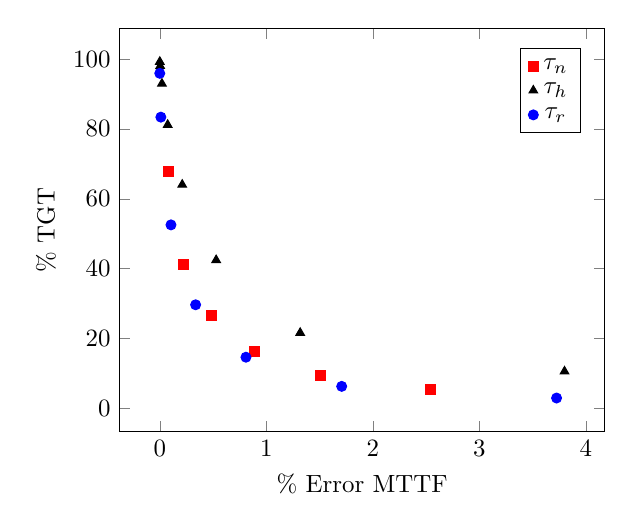
\begin{tikzpicture}[scale=0.9]
	    \begin{axis}[
	    	max space between ticks=30,
	        ylabel=\% TGT,
	        xlabel=\% Error MTTF,
            legend style={at={(0.95,0.95)},anchor=north east},
	      ]
	        \addplot[only marks,red,mark=square*] coordinates {
				%(36.2283821103523,	1.131498272)
				%(10.8786955953901,	2.0599948)
				%(4.71755048985506,	2.926328112)
				(2.53732952715346,	5.310854768)
				(1.50720646565421,	9.43458592)
				(0.889037571328778,	16.21424912)
				(0.482749275852648,	26.56263144)
				(0.227135116763804,	41.153888896)
				(0.080131519802844,	67.78028296)
	        };
	        \addlegendentry{$\tau_n$}
	        \addplot[only marks,black,mark=triangle*] coordinates {
				%(15.2851051823572,	5.065407888)
				(3.79933073326488,	10.55315872)
				(1.31806263244633,	21.607843456)
				(0.529240557949356,	42.444563712)
				(0.210743257691422,	64.033783088)
				(0.074347725814652,	81.17720832)
				(0.020278035133284,	92.977935568)
				(0.003661223540978,	98.040626224)
				(0.000329817987781,	99.235025232)
	        };
	        \addlegendentry{$\tau_h$}
	        \addplot[only marks,blue] coordinates {
	            %(53.6115397530694,	0.917438928)
				%(10.3724266177443,	1.873340144)
				(3.72475662384617,	2.934580832)
				(1.70774969809274,	6.27211712)
				(0.809117898074521,	14.623058272)
				(0.336501695329488,	29.640801488)
				(0.105215457995291,	52.52442624)
				(0.010279358713953,	83.38141984)
				(0.000009595371626,	95.930529824)
	        };
	        \addlegendentry{$\tau_r$}
	    \end{axis}
	\end{tikzpicture}
	\hspace{2em}
	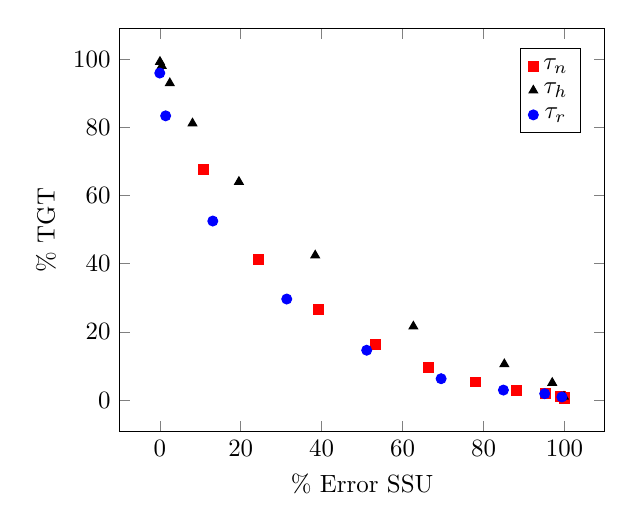
\begin{tikzpicture}[scale=0.9]
	    \begin{axis}[
	    	max space between ticks=30,
	        ylabel=\% TGT,
	        xlabel=\% Error SSU,
            legend style={at={(0.95,0.95)},anchor=north east},
	      ]
	        \addplot[only marks,red,mark=square*] coordinates {
		        (99.997820138894, 0.597874032)
				(99.9190691529866, 0.690664304)
				(98.9400899955787, 1.131498272)
				(95.4067719798257, 2.0599948)
				(88.2268633635062, 2.926328112)
				(78.0336186597343, 5.310854768)
				(66.3306911661053, 9.43458592)
				(53.4052347601024, 16.21424912)
				(39.2033637637174, 26.56263144)
				(24.49364613515, 41.153888896)
				(10.7288011862567, 67.78028296)
	        };
	        \addlegendentry{$\tau_n$}
	        \addplot[only marks,black,mark=triangle*] coordinates {
		        (99.870014762329, 1.004211856)
				(96.9670506258595, 5.065407888)
				(85.1329865668151, 10.55315872)
				(62.6536991241504, 21.607843456)
				(38.4026259662758, 42.444563712)
				(19.5569700042169, 64.033783088)
				(8.08755576023673, 81.17720832)
				(2.47742761181436, 92.977935568)
				(0.48941938798856, 98.040626224)
				(0.047212021885594, 99.235025232)
	        };
	        \addlegendentry{$\tau_h$}
	        \addplot[only marks,blue] coordinates {
	            (99.3410468520112, 0.917438928)
				(95.1059074056778, 1.873340144)
				(84.900750769067, 2.934580832)
				(69.5121048248012, 6.27211712)
				(51.1240231864542, 14.623058272)
				(31.3717210540309, 29.640801488)
				(13.1024452694744, 52.52442624)
				(1.45530814163918, 83.38141984)
				(0.001373917182918, 95.930529824)
	        };
	        \addlegendentry{$\tau_r$}
	    \end{axis}
	\end{tikzpicture}
	\captionof{figure}{Two graphs showing the relation between \% TGT and \%Error in MTTF/SSU}
	\label{fig:graph2}
\end{minipage}
\begin{document}
\noindent\begin{minipage}[c]{\textwidth}
	\centering
	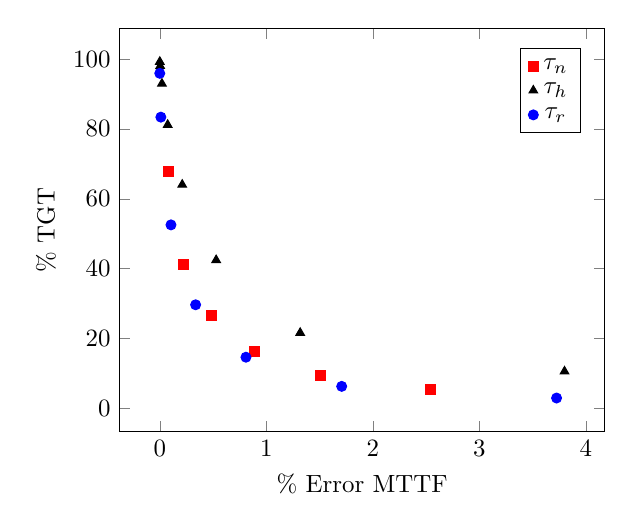
\begin{tikzpicture}[scale=0.9]
	    \begin{axis}[
	    	max space between ticks=30,
	        ylabel=\% TGT,
	        xlabel=\% Error MTTF,
            legend style={at={(0.95,0.95)},anchor=north east},
	      ]
	        \addplot[only marks,red,mark=square*] coordinates {
				%(36.2283821103523,	1.131498272)
				%(10.8786955953901,	2.0599948)
				%(4.71755048985506,	2.926328112)
				(2.53732952715346,	5.310854768)
				(1.50720646565421,	9.43458592)
				(0.889037571328778,	16.21424912)
				(0.482749275852648,	26.56263144)
				(0.227135116763804,	41.153888896)
				(0.080131519802844,	67.78028296)
	        };
	        \addlegendentry{$\tau_n$}
	        \addplot[only marks,black,mark=triangle*] coordinates {
				%(15.2851051823572,	5.065407888)
				(3.79933073326488,	10.55315872)
				(1.31806263244633,	21.607843456)
				(0.529240557949356,	42.444563712)
				(0.210743257691422,	64.033783088)
				(0.074347725814652,	81.17720832)
				(0.020278035133284,	92.977935568)
				(0.003661223540978,	98.040626224)
				(0.000329817987781,	99.235025232)
	        };
	        \addlegendentry{$\tau_h$}
	        \addplot[only marks,blue] coordinates {
	            %(53.6115397530694,	0.917438928)
				%(10.3724266177443,	1.873340144)
				(3.72475662384617,	2.934580832)
				(1.70774969809274,	6.27211712)
				(0.809117898074521,	14.623058272)
				(0.336501695329488,	29.640801488)
				(0.105215457995291,	52.52442624)
				(0.010279358713953,	83.38141984)
				(0.000009595371626,	95.930529824)
	        };
	        \addlegendentry{$\tau_r$}
	    \end{axis}
	\end{tikzpicture}
	\hspace{2em}
	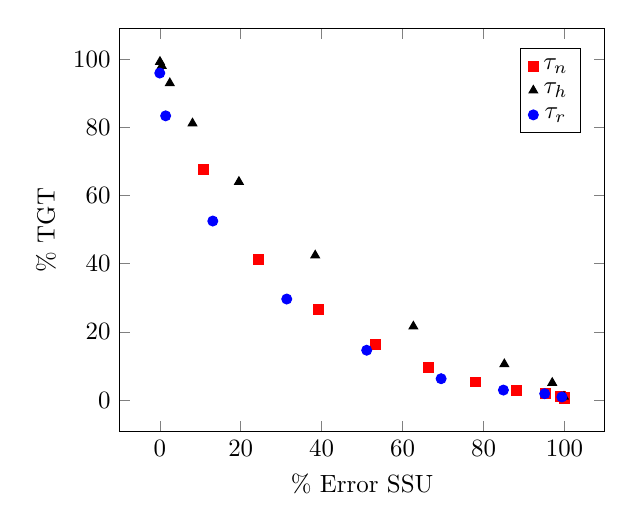
\begin{tikzpicture}[scale=0.9]
	    \begin{axis}[
	    	max space between ticks=30,
	        ylabel=\% TGT,
	        xlabel=\% Error SSU,
            legend style={at={(0.95,0.95)},anchor=north east},
	      ]
	        \addplot[only marks,red,mark=square*] coordinates {
		        (99.997820138894, 0.597874032)
				(99.9190691529866, 0.690664304)
				(98.9400899955787, 1.131498272)
				(95.4067719798257, 2.0599948)
				(88.2268633635062, 2.926328112)
				(78.0336186597343, 5.310854768)
				(66.3306911661053, 9.43458592)
				(53.4052347601024, 16.21424912)
				(39.2033637637174, 26.56263144)
				(24.49364613515, 41.153888896)
				(10.7288011862567, 67.78028296)
	        };
	        \addlegendentry{$\tau_n$}
	        \addplot[only marks,black,mark=triangle*] coordinates {
		        (99.870014762329, 1.004211856)
				(96.9670506258595, 5.065407888)
				(85.1329865668151, 10.55315872)
				(62.6536991241504, 21.607843456)
				(38.4026259662758, 42.444563712)
				(19.5569700042169, 64.033783088)
				(8.08755576023673, 81.17720832)
				(2.47742761181436, 92.977935568)
				(0.48941938798856, 98.040626224)
				(0.047212021885594, 99.235025232)
	        };
	        \addlegendentry{$\tau_h$}
	        \addplot[only marks,blue] coordinates {
	            (99.3410468520112, 0.917438928)
				(95.1059074056778, 1.873340144)
				(84.900750769067, 2.934580832)
				(69.5121048248012, 6.27211712)
				(51.1240231864542, 14.623058272)
				(31.3717210540309, 29.640801488)
				(13.1024452694744, 52.52442624)
				(1.45530814163918, 83.38141984)
				(0.001373917182918, 95.930529824)
	        };
	        \addlegendentry{$\tau_r$}
	    \end{axis}
	\end{tikzpicture}
	\captionof{figure}{Two graphs showing the relation between TGT and MTTF/SSU}
	\label{fig:graph2}
\end{minipage}


\iffalse
\begin{center}
	\begin{tabular}{|l|l|l|l|l|}
	\hline
    $\tau_h$  & Trees   & TGT (s) & MTTF   & SSU    \\ \hline
	3	&	1701	&	0.678	&	211.767	&	0.00485	\\ \hline
	4	&	21873	&	1.330	&	102.283	&	0.01220	\\ \hline
	5	&	80604	&	2.568	&	67.476	&	0.02012	\\ \hline
	6	&	161622	&	4.089	&	53.423	&	0.02628	\\ \hline
	7	&	236586	&	5.051	&	47.405	&	0.03003	\\ \hline
	8	&	287910	&	5.746	&	45.019	&	0.03186	\\ \hline
	9	&	312732	&	6.393	&	44.286	&	0.03251	\\ \hline
	10	&	320280	&	6.127	&	44.139	&	0.03266	\\ \hline
	11	&	321372	&	6.204	&	44.124	&	0.03267 \\ \hline
    \end{tabular}
\end{center}

\begin{center}
	\begin{tabular}{|l|l|l|l|l|}
	\hline
    $\tau_n$  & Trees   & TGT (s) & MTTF   & SSU    \\ \hline
    3	&	24	&	0.06	&	1642.68	&	0.0003	\\ \hline
	4	&	66	&	0.12	&	524.14	&	0.0015	\\ \hline
	5	&	192	&	0.16	&	252.28	&	0.0038	\\ \hline
	6	&	588	&	0.33	&	156.08	&	0.0071	\\ \hline
	7	&	1875	&	0.56	&	110.62	&	0.0110	\\ \hline
	8	&	6165	&	1.01	&	83.35	&	0.0152	\\ \hline
	9	&	20322	&	1.68	&	65.42	&	0.0198	\\ \hline
	10	&	63072	&	2.48	&	54.14	&	0.0246	\\ \hline
	11	&	167022	&	4.28	&	47.66	&	0.0291	\\ \hline
    \end{tabular}
\end{center}

\begin{center}
	\begin{tabular}{|l|l|l|l|l|}
	\hline
    $\tau_r$      & Trees  & TGT (s) & MTTF    & SSU    \\ \hline
    4E-1	&	18	&	0.06	&	2409.70	&	0.0002	\\ \hline
	8E-2	&	64	&	0.12	&	501.80	&	0.0015	\\ \hline
	16E-3	&	249	&	0.18	&	208.48	&	0.0049	\\ \hline
	32E-4	&	1142	&	0.38	&	119.48	&	0.0099	\\ \hline
	64E-5	&	5838	&	0.92	&	79.83	&	0.0159	\\ \hline
	128E-6	&	27955	&	1.85	&	58.97	&	0.0224	\\ \hline
	256E-7	&	105462	&	3.27	&	48.77	&	0.0284	\\ \hline
	512E-8	&	251637	&	5.31	&	44.58	&	0.0322	\\ \hline
	1024E-9	&	320861	&	6.22	&	44.12	&	0.0327	\\ \hline
    \end{tabular}
\end{center}

\begin{minipage}[c]{\textwidth}
	\centering
	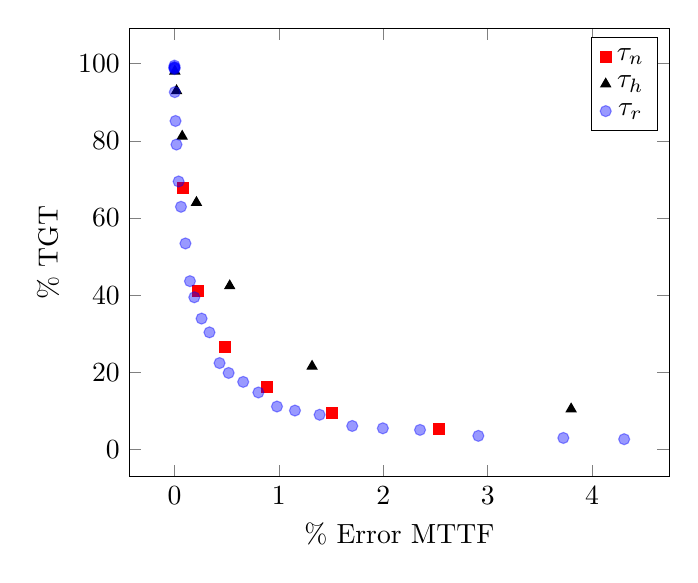
\begin{tikzpicture}
	    \begin{axis}[
	    	max space between ticks=30,
	        xlabel=\% Error MTTF,
	        ylabel=\% TGT
	      ]
	        \addplot[only marks,red,mark=square*] coordinates {
	            %(36.2283821103523, 1.131498272)
				%(10.8786955953901, 2.0599948)
				%(4.71755048985506, 2.926328112)
				(2.53732952715346, 5.310854768)
				(1.50720646565421, 9.43458592)
				(0.889037571328778, 16.21424912)
				(0.482749275852648, 26.56263144)
				(0.227135116763804, 41.153888896)
				(0.080131519802844, 67.78028296)
	        };
	        \addlegendentry{$\tau_n$}
	        \addplot[only marks,black,mark=triangle*] coordinates {
	            %(15.2851051823572, 5.065407888)
				(3.79933073326488, 10.55315872)
				(1.31806263244633, 21.607843456)
				(0.529240557949356, 42.444563712)
				(0.210743257691422, 64.033783088)
				(0.074347725814652, 81.17720832)
				(0.020278035133284, 92.977935568)
				(0.003661223540978, 98.040626224)
	        };
	        \addlegendentry{$\tau_h$}
	        \addplot[only marks,blue,opacity=0.4] coordinates {
%(77.8389169546306, 00.861523664)
%(53.6115397530694, 00.974922144)
%(36.9436300763677, 01.152995024)
%(19.6691222136954, 01.345055408)
%(12.7403247404829, 01.904005072)
%(10.3724266177443, 01.981527472)
%(8.03701794393446, 02.251020576)
%(5.44037121681866, 02.664600432)
(4.30725484221952, 02.719792576)
(3.72475662384617, 03.040657568)
(2.91070806039755, 03.582141952)
(2.3520596495621, 05.126460944)
(1.99594369221807, 05.54379928)
(1.70283035361238, 06.145844688)
(1.39021921620469, 09.046704608)
(1.15419515287708, 10.136940352)
(0.981883253585455, 11.18185456)
(0.803778142429072, 14.81874224)
(0.658367890409094, 17.559864032)
(0.51894407728556, 19.877736832)
(0.431973948594048, 22.436950304)
(0.335262945633125, 30.392851952)
(0.259775233206219, 33.959527536)
(0.190106610385051, 39.480168544)
(0.1484695504721, 43.655010816)
(0.105215457995291, 53.421811456)
(0.062484238182606, 62.918921632)
(0.039821874791978, 69.478455152)
(0.019324786397644, 79.03968496)
(0.010279358713953, 85.14784744)
(0.003281976729983, 92.620473392)
(0.000287846441507, 98.61676752)
(0.000074191212126, 98.965718112)
(0.000009595371626, 99.49783808)
(0.000001197524504, 99.10566392)
(0.000000113524206, 98.86297784)
	        };
	        \addlegendentry{$\tau_r$}
	    \end{axis}
	\end{tikzpicture}
	\captionof{figure}{Minute stepping in $\tau_r$ shows a clear improvement over any other $\tau$}
	\label{fig:graph3}
\end{minipage}

% 81 State
\begin{minipage}[c]{\textwidth}
	\centering
	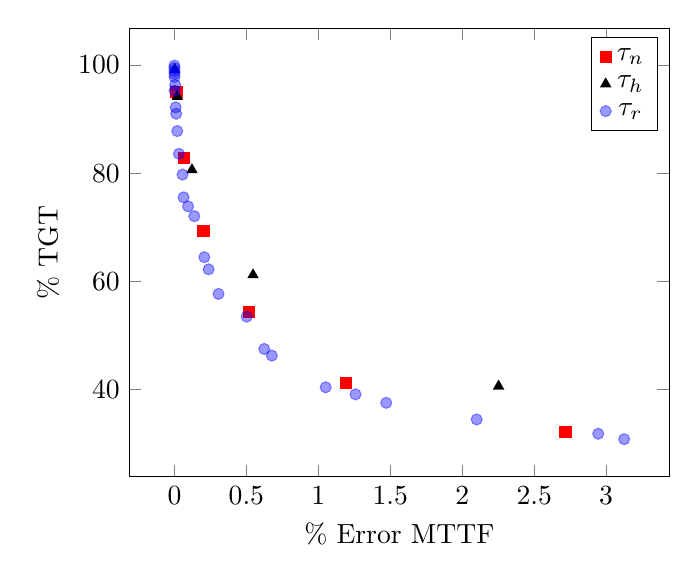
\begin{tikzpicture}
	    \begin{axis}[
	    	max space between ticks=30,
	        xlabel=\% Error MTTF,
	        ylabel=\% TGT
	      ]
	        \addplot[only marks,red,mark=square*] coordinates {
	            %(5.02356733929106,	30.6303230769231)
				(2.71781809857448,	32.1258746153846)
				(1.19345895314716,	41.2185853846154)
				(0.520816637597802,	54.3835530769231)
				(0.201764010931076,	69.2731269230769)
				(0.067155085775678,	82.8059223076923)
				(0.014209316034981,	95.0058284615385)
	        };
	        \addlegendentry{$\tau_n$}
	        \addplot[only marks,black,mark=triangle*] coordinates {
				(2.25246858832252,	40.5968253846154)
				(0.546184330425987,	61.1857253846154)
				(0.121706586210191,	80.6198246153846)
				(0.019773474449267,	94.1833223076923)
				(0.001247561153423,	99.1572384615385)
	        };
	        \addlegendentry{$\tau_h$}
	        \addplot[only marks,blue,opacity=0.4] coordinates {
	        	(3.12506926568685,	30.7972946153846)
				(2.94480631042475,	31.8045646153846)
				(2.10013178693072,	34.4441746153846)
				(1.47161276127877,	37.5233269230769)
				(1.25842149108485,	39.0925892307692)
				(1.05077091075744,	40.3940484615385)
				(0.6766517289396,	46.2565776923077)
				(0.624051517797217,	47.4933207692308)
				(0.50223924832624,	53.46519)
				(0.306166393081768,	57.6748276923077)
				(0.237358306879776,	62.2170792307692)
				(0.20738830622424,	64.4673376923077)
				(0.138260807577231,	72.0491353846154)
				(0.094839545585622,	73.8656815384616)
				(0.063323221521976,	75.5345892307692)
				(0.055950121488605,	79.7482407692308)
				(0.03117135243904,	83.5863061538462)
				(0.01955664092101,	87.7959569230769)
				(0.012331898334393,	91.0010630769231)
				(0.008335677618549,	92.1741538461539)
				(0.005181278438389,	96.3272938461538)
				(0.001099096032075,	95.2705438461539)
				(0.000795662048019,	98.3771769230769)
				(0.000211584918239,	97.7885453846154)
				(0.00017956152187,	98.9246561538462)
				(0.000023063648281,	99.4467030769231)
				(0.000001201233582,	99.9065630769231)
	        };
	        \addlegendentry{$\tau_r$}
	    \end{axis}
	\end{tikzpicture}
	\captionof{figure}{81-State Model}
\end{minipage}

% 1944 State
\begin{minipage}[c]{\textwidth}
	\centering
	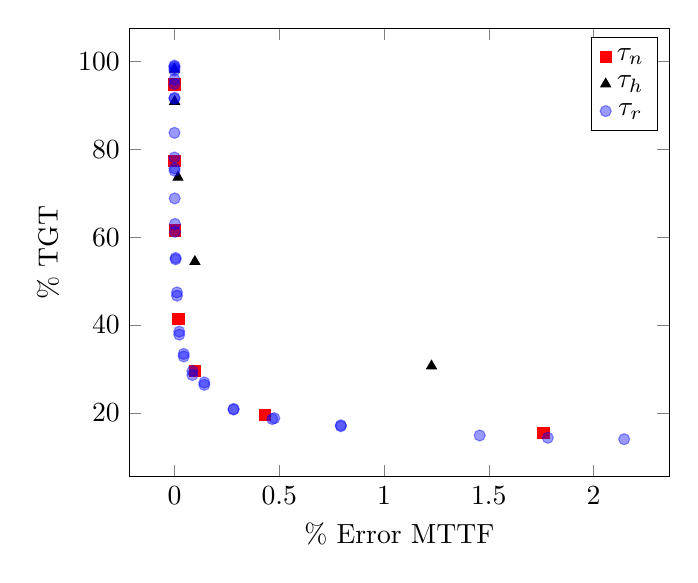
\begin{tikzpicture}
	    \begin{axis}[
	    	max space between ticks=30,
	        xlabel=\% Error MTTF,
	        ylabel=\% TGT
	      ]
	        \addplot[only marks,red,mark=square*] coordinates {
	            %100.046983929482	6.86980110497238
				%25.329782066667	8.32836184348556
				%(6.24701523124946,	10.9104475138122)
				(1.76139122714737,	15.4553731030142)
				(0.43051377054828,	19.4882542135814)
				(0.09826178843681,	29.5096597664172)
				(0.019692004739645,	41.427081404294)
				(0.003249002067894,	61.4902762430939)
				(0.000363538576137,	77.3120027274635)
				(0.000018509931622,	94.7138674732499)
	        };
	        \addlegendentry{$\tau_n$}
	        \addplot[only marks,black,mark=triangle*] coordinates {
	            %(55.2857697093697,	9.18041960976292)
				%(6.68456797207863,	15.0800960207008)
				(1.22671912255355,	30.6872349814672)
				(0.09749130661054,	54.4350767186517)
				(0.01689551149347,	73.57810630114)
				(0.000781590305106,	90.8398843275754)
				(0.000091030351497,	98.1599496468284)
	        };
	        \addlegendentry{$\tau_h$}
	        \addplot[only marks,blue,opacity=0.4] coordinates {
				%(44.3683164881073,	7.17263598853067)
				%(44.3683164881073,	6.9113154066718)
				%(25.2985330637396,	7.52712630253864)
				%(25.2985330637396,	7.62268305475908)
				%(17.2976450677203,	8.27936981607106)
				%(17.2976450677203,	8.04128820197217)
				%(8.44326796637061,	8.92883712147703)
				%(8.44326796637061,	9.33480746905378)
				%(6.1867869505139,	10.7300428701308)
				%(6.06069920242483,	10.7204565354221)
				%(3.835195371285,	12.0588028533464)
				%(3.835195371285,	11.5961596615148)
				(2.14605278739307,	14.0533783481362)
				(1.78168199273944,	14.3719619553815)
				(1.45675899768319,	14.8986251486118)
				(0.794015252752768,	16.9978301979159)
				(0.794015252752768,	17.217361004266)
				(0.47659370803887,	18.8331930904259)
				(0.466915201315304,	18.6260748304077)
				(0.282186265671425,	20.9209813973005)
				(0.282186265671425,	20.784251416183)
				(0.142421486808392,	26.944322120428)
				(0.142421486808392,	26.3997393524023)
				(0.085666349634763,	28.641364640884)
				(0.085666349634763,	29.5529364990559)
				(0.044235799257879,	32.8614357647388)
				(0.044085773867704,	33.4480611930904)
				(0.022828028933692,	37.8174917826421)
				(0.022828028933692,	38.5073814952095)
				(0.012277241930892,	46.6821288201972)
				(0.011957515876246,	47.4230330792363)
				(0.005546322895692,	54.9514041541367)
				(0.005539907234219,	55.2649633540807)
				(0.002710672096611,	61.2008221553955)
				(0.002442241193297,	62.997692006434)
				(0.001155852212705,	68.797281418281)
				(0.000485709906838,	75.0943899573397)
				(0.000434170604007,	75.6398816700469)
				(0.000316107953914,	78.1029320232184)
				(0.000166891106412,	83.7073589761522)
				(0.000045210951517,	91.6875845863347)
				(0.000044449504197,	91.4417286523533)
				(0.000018699618874,	94.8065601790335)
				(0.000011798640481,	95.8290994475138)
				(0.000002230253202,	97.9071140639206)
				(0.000002230253202,	98.4095240925939)
				(0.000000081224462,	98.9988306175257)
				(0.000000081224462,	98.7697962794601)
	        };
	        \addlegendentry{$\tau_r$}
	    \end{axis}
	\end{tikzpicture}
	\captionof{figure}{1944-State Model}
\end{minipage}
\fi

\end{document}